\newpage % Rozdziały zaczynamy od nowej strony.
\cleardoublepage % Zaczynamy od nieparzystej strony
\pagestyle{headings}
\section{Wstęp}

\subsection{Wprowadzenie}

W ostatnich latach można zaobserwować gwałtowny rozwój w dziedzinie 
Uczenia Maszynowego (ang. \emph{Machine Learning}) i Sztucznej Inteligencji 
(ang. \emph{Artificial Intelligence}). Coraz więcej urządzeń i systemów projektowanych jest w sposób zapewniający działanie autonomicznie, bez potrzeby ingerencji człowieka. 
Jednym z algorytmów, który powstał już dość dawno, są Sztuczne Sieci Neuronowe (ang. \emph{Artificial Neural Networks}). Temat Sieci Neuronowych ma długą historię rozwoju, sięgającą początku lat 40. XX wieku, jednak w ostatnich latach można zaobserwować znaczny postęp w tej dziedzinie \cite{Kriesel2007NeuralNetworks}. Rozwój technologii umożliwił zastosowanie algorytmów AI w wielu aplikacjach. Działalność naukowa w kierunku Sztucznych Sieci Neuronowych spowodowała powstanie nowych modeli i architektur.

Większość algorytmów wykorzystujących Sztuczną Inteligencję wymaga dużej mocy 
obliczeniowej i wyboru odpowiedniego sprzętu. Często powtarzaną operacją matematyczną 
w przypadku algorytmu Sztucznej Sieci Neuronowej jest mnożenie macierzy.
Działanie to można w łatwy sposób zrównoleglić, implementując sieć w układzie 
FPGA i tym samym zwiększyć efektywność algorytmu.

Praca nad implementacją algorytmów Sztucznej Inteligencji w większości 
przypadków zaczyna się od stworzenia i uruchomienia modelu. Do tego zadania 
często wykorzystywane są wysokopoziomowe biblioteki takie jak \emph{keras} lub \emph{Theano}, które w znacznym stopniu przyspieszają proces tworzenia oprogramowania oraz ułatwiają wprowadzanie zmian w modelu sieci. Rozwój i dopracowywanie 
algorytmu Sztucznej Inteligencji wymaga wielu iteracji uruchamiania kodu 
z różnymi parametrami i właściwościami sieci. Aby w~pełni wykorzystać potencjał Sztucznych Sieci Neuronowych, należy dobrać odpowiednio metody projektowania i testowania modeli.

\subsection{Wstęp teoretyczny}

Sieć neuronowa jest algorytmem przetwarzającym dane, inspirowanym działaniem mózgu. ANN składa się z wielu elementów przetwarzających informacje -- neuronów. Model przetwarzania informacji jest inspirowany ludzkim mózgiem jednak w stosunku do komórki nerwowej, neuron w Sztucznej Sieci Neuronowej jest bardzo uproszczony
\cite{tadeusiewicz1993sieci}. Pomimo to ANN umożliwiają rozwiązywanie złożonych
problemów w wielu dziedzinach z~dużą dokładnością.

Pomiędzy neuronami prowadzone są połączenia, z których każde ma swoją wagę, która 
zmienia wartość w trakcie uczenia sieci. Warstwę sieci, w której wszystkie wyjścia każdego z neuronów są podłączone do wszystkich neuronów w warstwie następnej, nazywa się warstwą w pełni połączoną (ang. FC — \emph{Fully Connected}).
Sieć posiadająca wszystkie warstwy w pełni połączone jest zwana siecią w pełni połączoną. 

W znacznej większości sieci neuronowe budowane są w ten sposób, że dane są propagowane w kierunku od warstwy wejściowej do wyjściowej. Takie sieci nazywamy sieciami jednokierunkowymi (ang. \emph{feedforward}). Przykładową sieć neuronową w pełni połączoną typu \emph{feedforward} przedstawiono na Rys. \ref{ann-img}.
\bigskip

\begin{figure}[h]
  \centering
  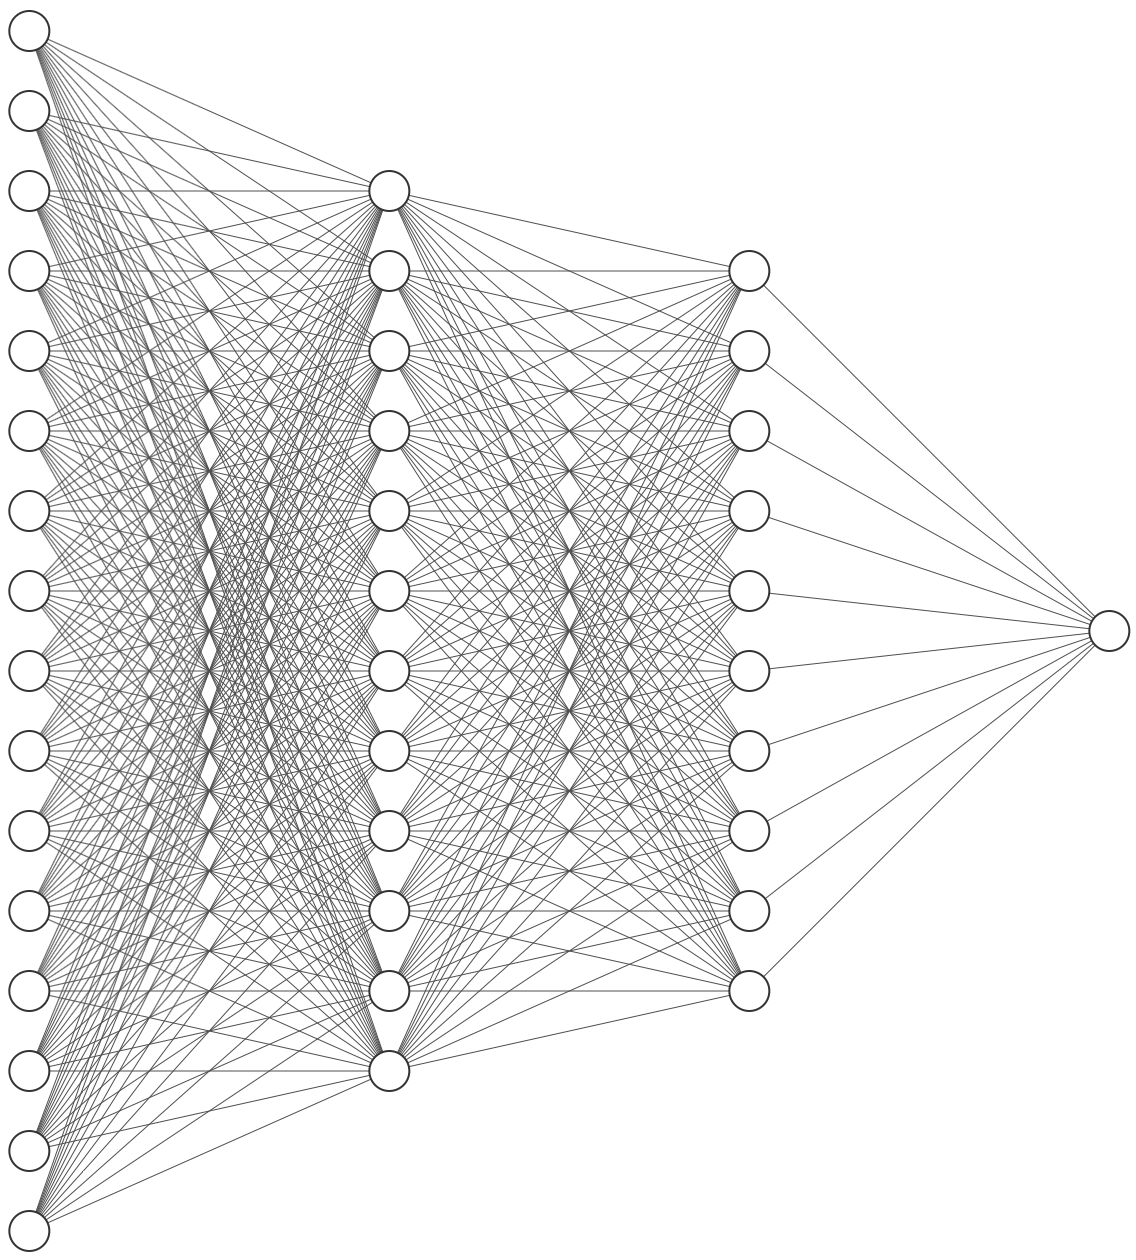
\includegraphics[width=0.8\textwidth]{img/ann.png}
  \caption{Schemat w pełni połączonej jednokierunkowej Sieci Neuronowej (wygenerowany na stronie: \url{http://alexlenail.me/NN-SVG/})}
  \label{ann-img}
\end{figure}


\subsubsection{Model neuronu}
Sztuczne Sieci Neuronowe to algorytm inspirowany działaniem ludzkiego mózgu 
i~znajdujących się w nim neuronów. Model matematyczny (Rys. \ref{neuron}) pojedynczego neuronu składa się z następujących elementów \cite{Omondi2006FPGAIO}:
\begin{itemize}
  \item wektora wejściowego: 
  $$x = (x_1, x_2,...,x_j)^T$$
  \item wektora wag przypisanych do każdego z wejść
  $$w = (w_{k1}, w_{k2},...,w_{kj})^T$$
  \item wyrazów wolnych (bias) $b$
  \item funkcji aktywacji $\phi(u)$ 
  \item wyjścia neuronu $y$. 
\end{itemize}
Wyrazy wolne (bias) umożliwiają kontrolowanie progu aktywacji neuronu, niezależnie od wartości wejściowych. W praktyce oznacza to przesuwanie wykresu funkcji aktywacji w~zależności od znaku w prawą lub w lewą stronę. Wyjście neuronu można policzyć, stosując następujące wzory:
$$u_k = \sum_{j=1}^{N}{w_{kj}x_j} $$ 
$$y_k = \phi(u_k + b_k) $$ 

Najprostsza Sieć Neuronowa składająca się z jednego neuronu, nazywana jest \emph{Perceptronem}. Algorytm ten można wykorzystać do zadań klasyfikacji binarnej.

\begin{figure}[h]
  \centering
  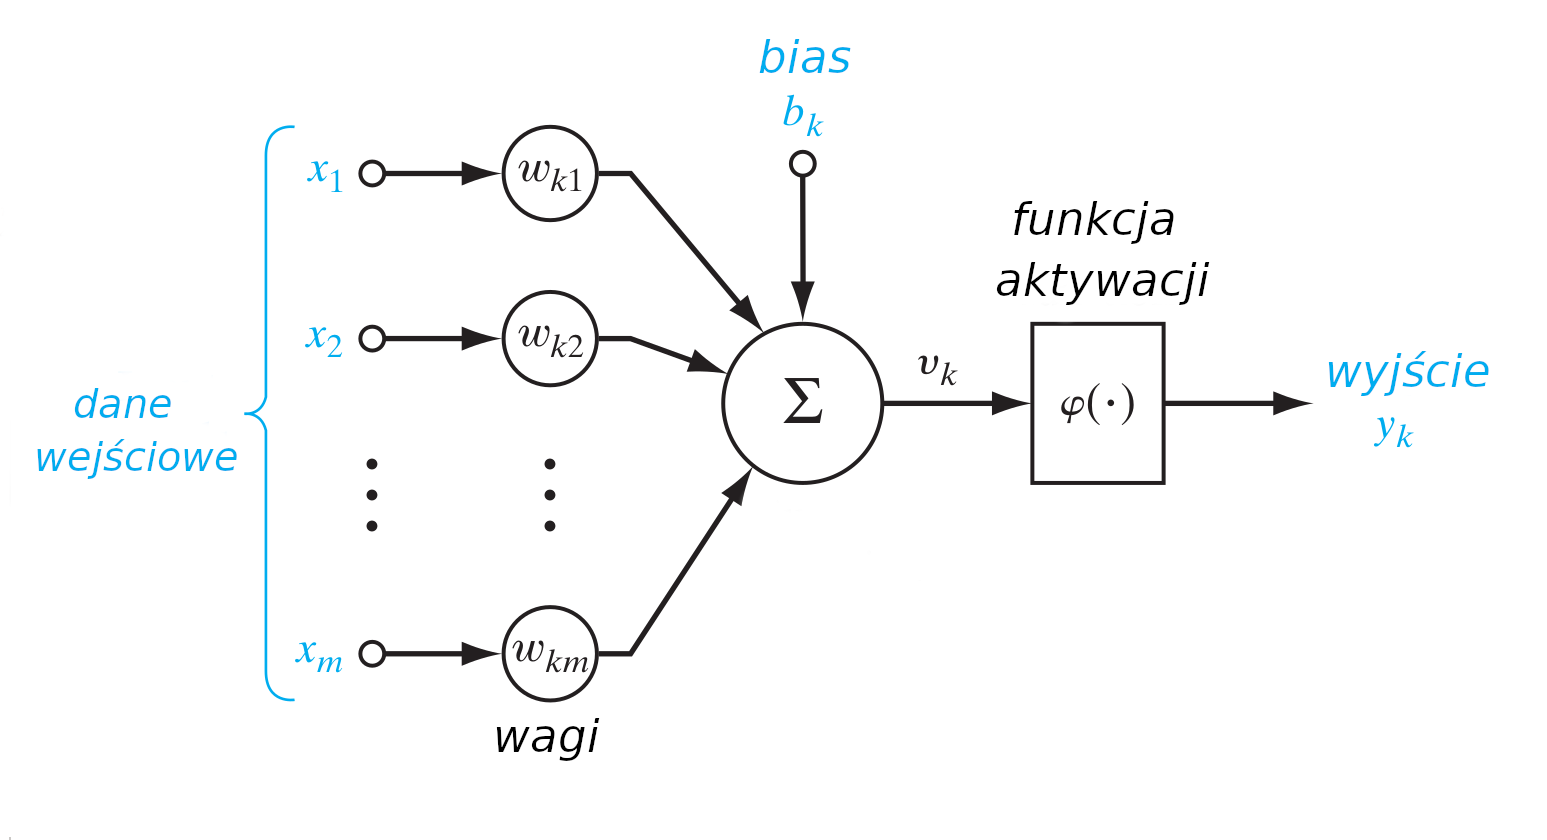
\includegraphics[width=\textwidth]{img/neuron.png}
  \caption{Model neuronu \cite{haykin2009neural}}
  \label{neuron}
\end{figure}


\subsubsection{Funkcja aktywacji}
Na działanie algorytmu znaczny wpływ może mieć dobór odpowiedniej 
funkcji aktywacji. Wśród najczęściej stosowanych funkcji aktywacji
wyróżnia się następujące funkcje:
\begin{itemize}
    \item funkcja ReLu (ang. \emph{Rectified Linear Units}): 
    
    $$\phi(x) = max(0, x)$$
    
    \begin{figure}[!h]
      \centering
      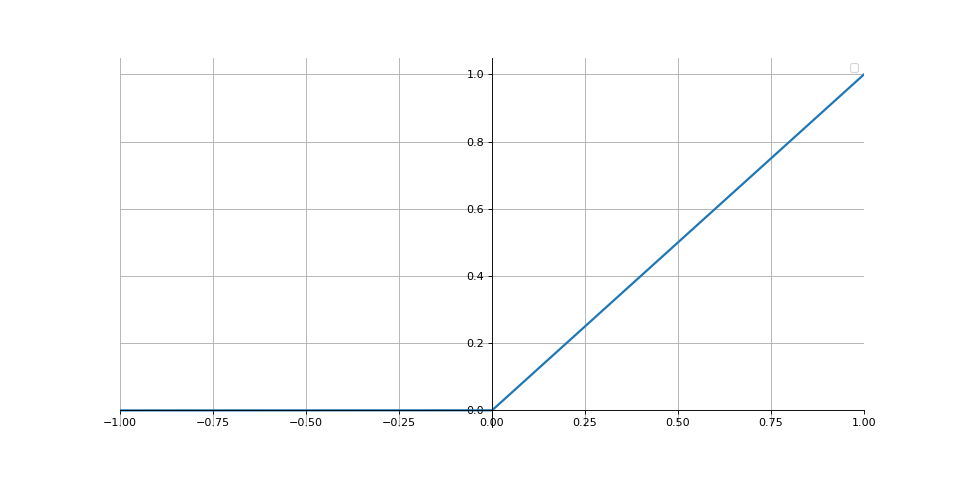
\includegraphics[width=\textwidth]{img/relu.png}
      \caption{Wykres funkcji ReLU}
      \label{relu}
    \end{figure}

    \item funkcja sigmoid: 
    
    $$\phi(x) = \frac{a}{a + e^{-bx}}$$
    
    \begin{figure}[!h]
      \centering
      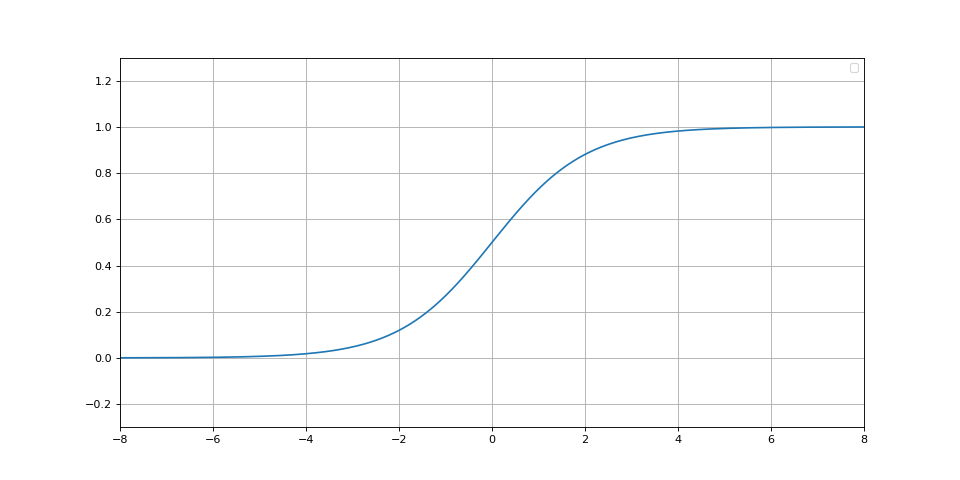
\includegraphics[width=\textwidth]{img/sigmoid.png}
      \caption{Wykres funkcji sigmoid}
      \label{sigmoid}
    \end{figure}
    
    \item funkcja softmax (liczona dla każdego neuronu warstwy wyjściowej, j = 1,...,N): 
    $$\phi(x_j) = \frac{e^{x_j}}{\sum_{k=1}^{N}{e^{x_k}}}$$
\end{itemize}

W warstwach ukrytych często używaną funkcją aktywacji jest funkcja ReLU oraz sigmoid. Funkcję sigmoid stosuje się również w warstwach wyjściowych przy zadaniach klasyfikacji binarnej. Funkcja softmax jest używana w problemach klasyfikacji wieloklasowej (np. rozpoznawanie cyfr). Stosując funkcję softmax w warstwie wyjściowej, można traktować wektor wartości wyjść sieci jako rozkład prawdopodobieństwa wyboru danego rozwiązania.

\subsubsection{Perceptron wielowarstwowy}
Jednym z pierwszych modeli Sztucznych Sieci Neuronowych był Perceptron
Wielowarstwowy (ang. MLP — \emph{Multi-Layer Perceptron}), składający 
się z warstwy neuronów wejściowej, ukrytych i wyjściowej (Rys.\ref{mlp}).
Wyjście neuronów w danej warstwie staje się wejściem neuronów warstwy następnej.

Sieć Neuronowa typu MLP najczęściej posiada warstwy w pełni połączone
(ang. FC -- \emph{Fully Connected}) lub inaczej Gęste (ang. \emph{Dense}). W warstwie FC każde z wyjść jest podłączone do wszystkich wejść neuronów w warstwie następnej.

\begin{figure}[h]
  \centering
  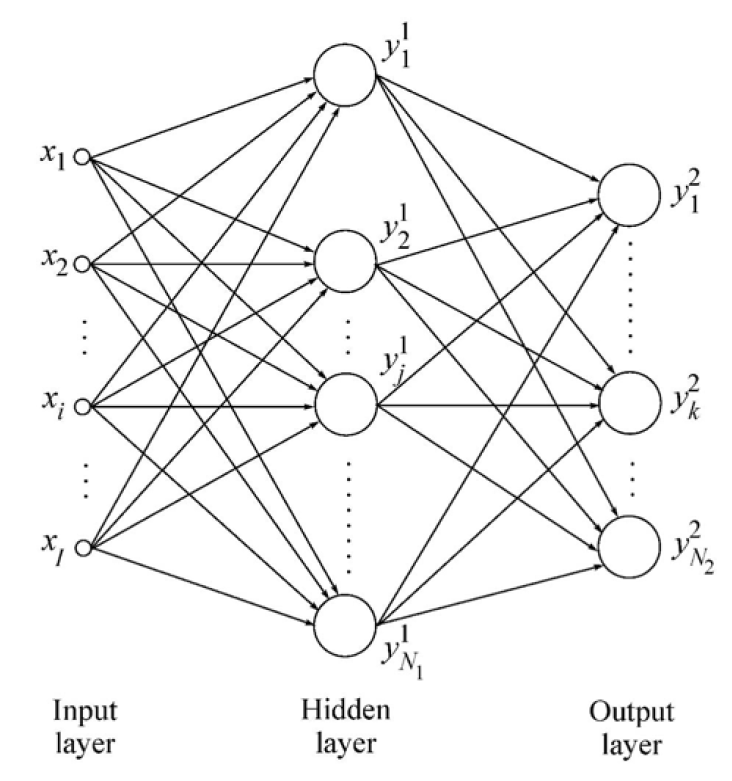
\includegraphics[width=\textwidth]{img/mlp.png}
  \caption{Model Perceptronu Wielowarstwowego}
  \label{mlp}
\end{figure}


\subsubsection{Sieci Głębokie}

Rozwój algorytmów AI doprowadził do powstania Głębokich Sieci Neuronowych (ang. 
\emph{DNN — Deep Neural Networks}), czyli takich, które posiadają wiele 
warstw ukrytych \cite{Goodfellow-et-al-2016}. Algorytm Uczenia Głębokiego (ang. 
\emph{Deep Learning}) umożliwia rozwiązywanie skomplikowanych problemów takich 
jak rozpoznawanie i klasyfikację obiektów na obrazie (Rys.\ref{dnn}). Seria warstw ukrytych (ang. \emph{hidden layers}) umożliwia ekstrakcję cech obiektów. 
Kolejne warstwy umożliwiają wykrywanie krawędzi, potem konturów, a na końcu 
całych kształtów i obiektów.

\begin{figure}[!h]
  \centering
  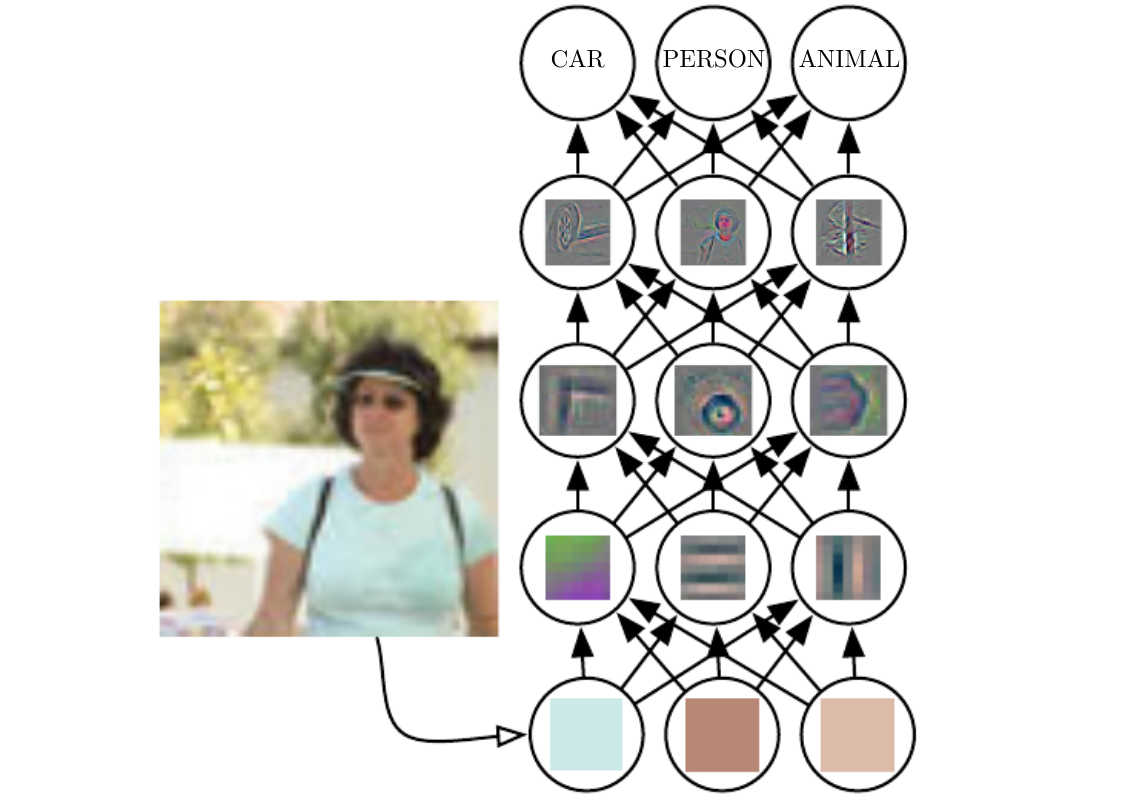
\includegraphics[width=\textwidth]{img/dnn-object-recog.png}
  \caption{Model Głębokiego Uczenia sieci \cite{Goodfellow-et-al-2016}}
  \label{dnn}
\end{figure}


\subsubsection{Proces uczenia sieci}

Uczenie Sztucznej Sieci Neuronowej można podzielić na nadzorowane (ang. \emph{supervised learning}) i nienadzorowane (ang. \emph{unsupervised learning}) oraz wersję pośrednią -- uczenie częściowo nadzorowane (ang. \emph{semi-supervised learning}). W praktyce najczęściej wykorzystywanym rodzajem uczenia jest \emph{supervised learning}, jednak uczenie nienadzorowane, które zakłada tworzenie modelu sieci bez ingerencji człowieka, jest ciekawym tematem badań i rozwoju algorytmów Sztucznych Sieci Neuronowych \cite{nielsen2015neural}.
Proces uczenia nadzorowanego sieci polega na zwiększaniu dokładności ANN w rozwiązywaniu danego problemu. Odbywa się to poprzez iteracyjne korygowanie wartości wag i wyrazów wolnych (bias) tak, aby zminimalizować błąd pomiędzy rozwiązaniem wzorcowym i otrzymanym. Jeden z algorytmów zmiany wag podczas uczenia jest reguła delty (ang. \emph{delta rule}):


$$\Delta w_{kj} = \eta e_k(n)x_j(n) $$
$$ e_k(n) = d_k(n) - y_k(n) $$

W powyższym wzorze $d_k(n)$ jest zakładanym rozwiązaniem, a $y_k(n)$ rozwiązaniem otrzymanym.
Wartość $\eta$ oznacza współczynnik szybkości uczenia (ang. \emph{learning rate}). Gdy jest wystarczająco mały, algorytm uczenia osiąga rozwiązanie optymalne, jednak większy współczynnik $\eta$ może przyspieszyć ten proces. Wpływ na szybkość uczenia ma również wielkość miniserii (ang. \emph{mini-batch}) uczących. Jest to liczba elementów zbioru uczącego, podawanych na wejście algorytmu, przed zaktualizowaniem wartości wag sieci. Z powodu ograniczonych rozmiarów zboru uczącego, jest on wykorzystywany wielokrotnie. Jedno przejście przez wszystkie próbki ze zbioru uczącego nazywane jest epoką (ang. \emph{epoch}) \cite{tadeusiewicz2015leksykon}.

\subsubsection{Wsteczna propagacja błędu}
Architekturę sieci MLP często stosuje się wraz z algorytmem wstecznej 
propagacji błędu (ang. \emph{Backpropagation}), która umożliwia proces uczenia sieci. Poprzez obliczenie błędu w neuronach warstwy wyjściowej i propagacji wstecz błędu przez całą sieć, algorytm pozwala dostosować wartość wagi każdego z połączeń w taki sposób, aby zminimalizować wartość funkcji kosztu. Sieć jest uczona do momentu, gdy błąd stanie się akceptowalnie mały. 

\subsubsection{Hiperparametry}
W procesie uczenia Sztucznej Sieci Neuronowej bardzo istotne jest odpowiednie ustawienie parametrów sieci, zwanych hiperparametrami (ang. \emph{hyperparameters}). Są to parametry sieci, ustawiane przez użytkownika w celu otrzymania modelu, dającego najlepsze rozwiązania. Na wynik uczenia wpływ mają m.in. następujące Hiperparametry:
\begin{itemize}
  \item liczba i rodzaj warstw sieci
  \item liczba neuronów w każdej z warstw
  \item współczynnik szybkości uczenia $\eta$
  \item wielkość miniserii
  \item liczba epok.
\end{itemize}

\subsubsection{Przeuczenie sieci}

Przy używaniu Sztucznych Sieci Neuronowych w zadaniach klasyfikacji często spotykanym problemem jest przeuczenie sieci (ang. \emph{overfitting}). Przeuczona sieć jest zbyt mocno dopasowana do danych uczących i przy walidacji poprawność klasyfikacji jest znacznie mniejsza. Jednym ze sposobów na polepszenie zdolności do generalizacji trenowanego modelu sieci jest zastosowanie \emph{Dropoutu}, czyli losowego usuwania pewnej ustalonej liczby neuronów. Technika ta, pomimo swojej prostoty, daje bardzo dobre wyniki w~przeciwdziałaniu przeuczeniu sieci.  

\subsubsection{Splotowe Sieci Neuronowe}

Splotowe Sieci Neuronowe (ang. \emph{CNN -- Convolutional Neural Networks}) są typem sieci głębokich, które znakomicie nadają się do rozpoznawania kształtów i z powodzeniem stosowane w wielu zagadnieniach klasyfikacji obrazów. Charakteryzują się dużą odpornością na rotację, skalowanie, zniekształcanie i inne zakłócenia \cite{haykin2009neural}. Sieci te są uczone w trybie nadzorowanym. 

Za ekstrakcję cech obiektów w dwuwymiarowym obrazie odpowiedzialna jest warstwa splotowa sieci. Wejście \textbf{\emph{M}} tej warstwy jest przekształcane przy użyciu odpowiedniego filtru \textbf{\emph{K}}. Operację splotu w sieciach CNN można opisać wzorem:
$$
S(i,j) = (M*K)(i,j) =\sum_{k}{\sum_{j}{M(i - k, j - l)K(k, l)}}
$$

Wynik \textbf{\emph{S(i,j)}} nazywany jest mapą atrybutów (ang. \emph{feature map}). Warstwa splotowa umożliwia zmniejszenie rozmiaru przetwarzanych danych podczas uczenia sieci oraz zwiększa jej zdolność do generalizacji. Operację splotu przedstawiono na Rys. \ref{conv}. Zaprezentowany przypadek to splot macierzy 6x6 przy użyciu filtru o rozmiarze 3x3. 


\begin{figure}[!h]
  \centering
  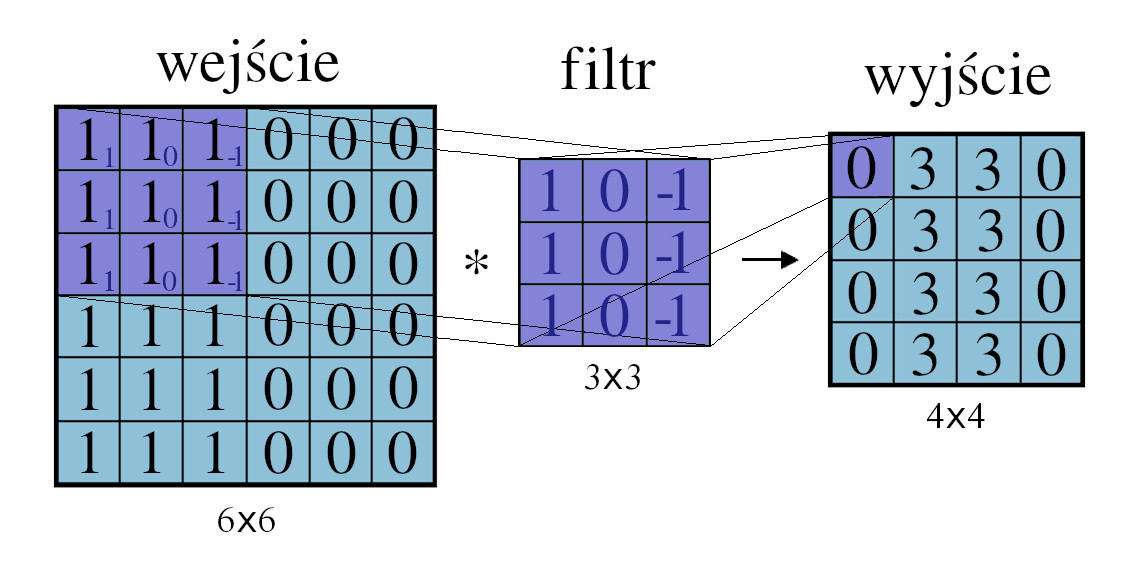
\includegraphics[width=\textwidth]{img/conv.jpg}
  \caption{Splot macierzy 6x6 przy użyciu filtru o rozmiarze 3x3}
  \label{conv}
\end{figure}


Razem z warstwą splotową często stosowana jest warstwa grupowania (ang. \emph{pooling}), występującą najczęściej w jednym z dwóch wariantów (ang. \emph{max-pooling}) lub (ang. \emph{average pooling}). W przypadku przetwarzania obrazu metoda (ang. \emph{max-pooling}) polega na zmniejszeniu jego rozmiaru, poprzez wybranie wartości maksymalnej lub średniej, stosując okno o wybranym rozmiarze. Najczęściej wybieranym krokiem (ang. \emph{stride}) przesuwania okna jest wartość, równa jego rozmiarowi. Na Rys. \ref{pooling} przedstawiono przykład \emph{max-poolingu} o rozmiarze 2x2 ze skokiem równym rozmiarowi okna.

\begin{figure}[!h]
  \centering
  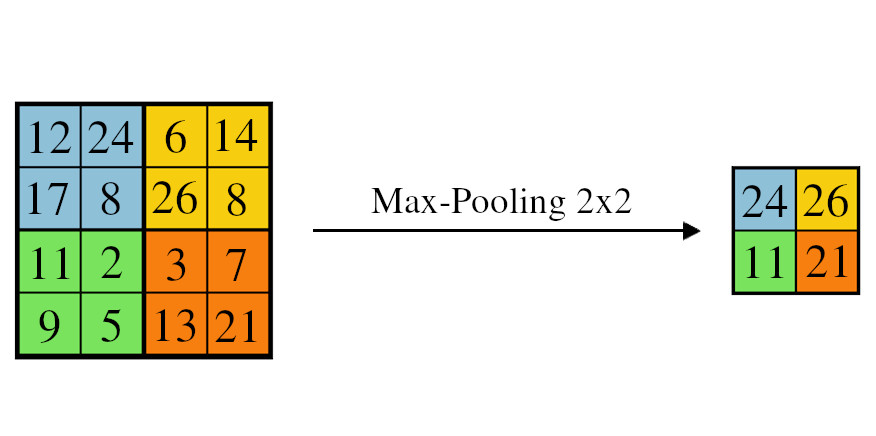
\includegraphics[width=\textwidth]{img/pooling.jpg}
  \caption{Max-pooling o rozmiarze 2x2}
  \label{pooling}
\end{figure}

\subsection{Zastosowania Sztucznych Sieci Neuronowych}

W dzisiejszych czasach Sztuczne Sieci Neuronowe są wykorzystywane w wielu zastosowaniach. Dziedziny, w których stosuje się algorytmy ANN to m.in.:
\begin{itemize}
  \item medycyna -- wspomaganie wystawiania diagnozy
  \item przemysł -- automatyczna kontrola jakości produktów
  \item zastosowania militarne -- wspomaganie radarów i termowizji
  \item ekonomia -- przewidywanie notowań giełdowych
  \item robotyka -- autonomiczne samochody (Rys. \ref{self-driving-car})
  \item rozpoznawanie i synteza mowy -- sterowanie różnymi systemami (smartfon, komputer, urządzenia IoT) przy użyciu asystenta głosowego
\end{itemize}

\begin{figure}[!h]
  \centering
  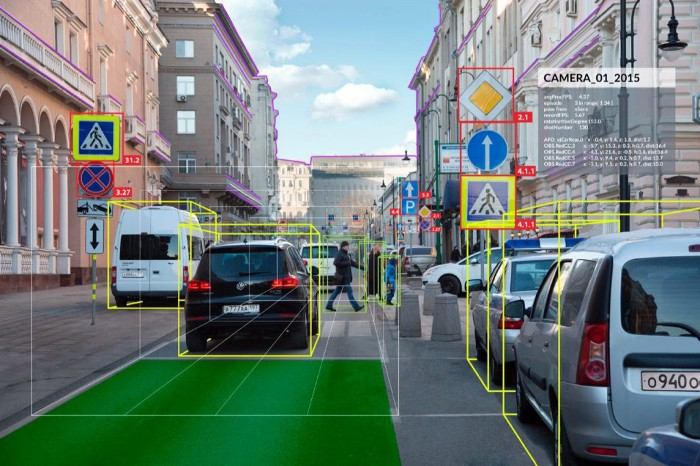
\includegraphics[width=\textwidth]{img/self-driving-car.jpg}
  \caption{Rozpoznawanie obiektów na obrazie z kamery samochodu autonomicznego \cite{self-drive-obraz}}
  \label{self-driving-car}
\end{figure}

